\chapter{Fugaの実装}
\ref{chap:design}章で述べたFugaの設計をもとにFugaを実装した.
本稿の実装は,TMP節で述べたケースの実例として,OpenSSLを利用して暗号化を行うランサムウェアを対象としている.
カーネル空間のプログラムはeBPF \cite{WhatiseB81:online} を利用して,
ユーザ空間のプログラムはGo言語を用いて実装した.
本稿の執筆時点においてeBPFは実用上Linux環境のみで利用可能であるため,
Linux環境にて実装を行った.
実装に使用したシステムの環境を\tabref{tab:impl-env}に示す.
\begin{table}[tb]
  \caption{Implementation environment for Fuga.}
  \label{tab:impl-env}
  \hbox to\hsize{\hfil
    \begin{tabular}{l|lll}
      \hline
      Linuxカーネル  & 6.3.0-060300-generic \\
      CPUアーキテクチャ & amd64                \\
      clang      & 14.0.0-1ubuntu1.1    \\
      Goコンパイラ    & go1.22.5 linux/amd64 \\
    \end{tabular}\hfil}
\end{table}

\section{各コンポーネントの実装}
本節ではFugaの実装特有の詳細を説明する.
Detectorの実装は本研究のスコープ外であることに注意する.

\subsection{Process Monitor}
\subsubsection{Capturer}
Capturerは,OpenSSL内の暗号化関数をuprobeでフックするeBPFプログラムとして実装した.
暗号化関数には引数として平文データが格納されているバッファへのポインタが渡されるため,
eBPFプログラム内でこのポインタをキャプチャしユーザ空間からカーネル空間へ平文データをコピーする.
コピーされた平文データは,関連するメタデータとともに暗号化イベントを表す構造体に格納され,
eBPF mapのリングバッファを介してEvacuation Moduleに送信される.
なお,本稿で示す実装においてはOpenSSLの暗号化関数のみを対象としているが,
OpenSSL以外の暗号化ライブラリにも容易に同じ手法を適用することができる.

\subsubsection{Collector}
CollectorはCapturerが取得した平文データに対して,
元ファイルの絶対パスと元ファイル上のオフセットを取得する機能を持つ.
上述したようにCollectorがアクセスできるのは平文データのポインタのみであり,ポインタから絶対パスやオフセットを直接取得することはできない.
そこで本研究では,FD (File Descriptor) を仲介して必要なデータを取得する方法を採用した.
\texttt{read(2)}システムコールはFDとバッファのポインタを引数として受け取るため,
\texttt{read(2)}をフックすることでポインタとFDの対応関係を取得することができる.
この対応関係を参照し,
\texttt{open(2)}システムコール (FDを返り値として戻す) のフックから相対または絶対パスを,
\texttt{lseek(2)}および\texttt{read(2)}システムコール (FDを引数に取り,FDに紐づくファイルのオフセットを更新する) のフックからオフセットを取得可能である.
\texttt{open(2)}, \texttt{read(2)}, \texttt{lseek(2)}の関数シグネチャを\coderef{code:syscalls}に示す.
より詳細には,以下の手順でFDの値から元ファイルの絶対パスとオフセットを取得する.
\\
\\
\textbf{元ファイルの絶対パス}:
\texttt{open(2)}のフックによりFDとファイルパスの関係が得られるので,
FDをkeyとし,ファイルパスをvalueとするハッシュマップにこの関係を保存する.
\texttt{open(2)}に渡された引数が相対パスであった場合,プロセスのCWD (Current Working Directory) と結合して絶対パスを取得する.
CWDはLinuxカーネルにおいて各ユーザプロセスの状態を管理するカーネル内変数である\texttt{task\_struct}を介して取得する.
\\
\textbf{元ファイル上のオフセット}:
\texttt{lseek(2)}および\texttt{read(2)}システムコールをフックする.
これらのシステムコールはFDを引数に取り,\texttt{lseek(2)}はシステムコール完了時のオフセットを,
\texttt{read(2)}はシステムコールによって読み込まれたバイト数を返す.
この性質を利用して,FDをkeyとし,オフセットをvalueとするハッシュマップにオフセットを保存する.
\texttt{open(2)}のフックによりファイルが開かれた際にハッシュマップにkey = 0, value = FD のエントリを追加しておき,
\texttt{lseek(2)}および\texttt{read(2)}が実行された際にvalueを更新しておく.

\begin{lstlisting}[caption=Signatures of the related system calls. The comment lines indicate the return value on success / error., label=code:syscalls, language=C]
  // a file descriptor / -1
  int open(const char *pathname, int flags, ...
        /* mode_t mode */ );
        
  // the number of bytes read / -1
  ssize_t read(int fd, void buf[.count], size_t count);

  // the resulting offset location in bytes / -1
  off_t lseek(int fd, off_t offset, int whence);
\end{lstlisting}


\subsection{Evacuation Module}
Evacuation Moduleは,Process Monitorによってリングバッファにデータが書き込まれるたびに呼び出しを行い,
平文データ,元ファイルの相対パスとCWD,オフセットを取得する.
その後絶対パスを構成し,絶対パスで指定されるファイルがData Shelter内に存在しなければ設計で示したようにファイルを作成する.
そしてオフセットで指定される位置に平文データを書き込む.
\figref{fig:evac-mon-impl}にEvacuation Moduleの実装を示す.
\begin{figure}[t]
  \begin{center}
    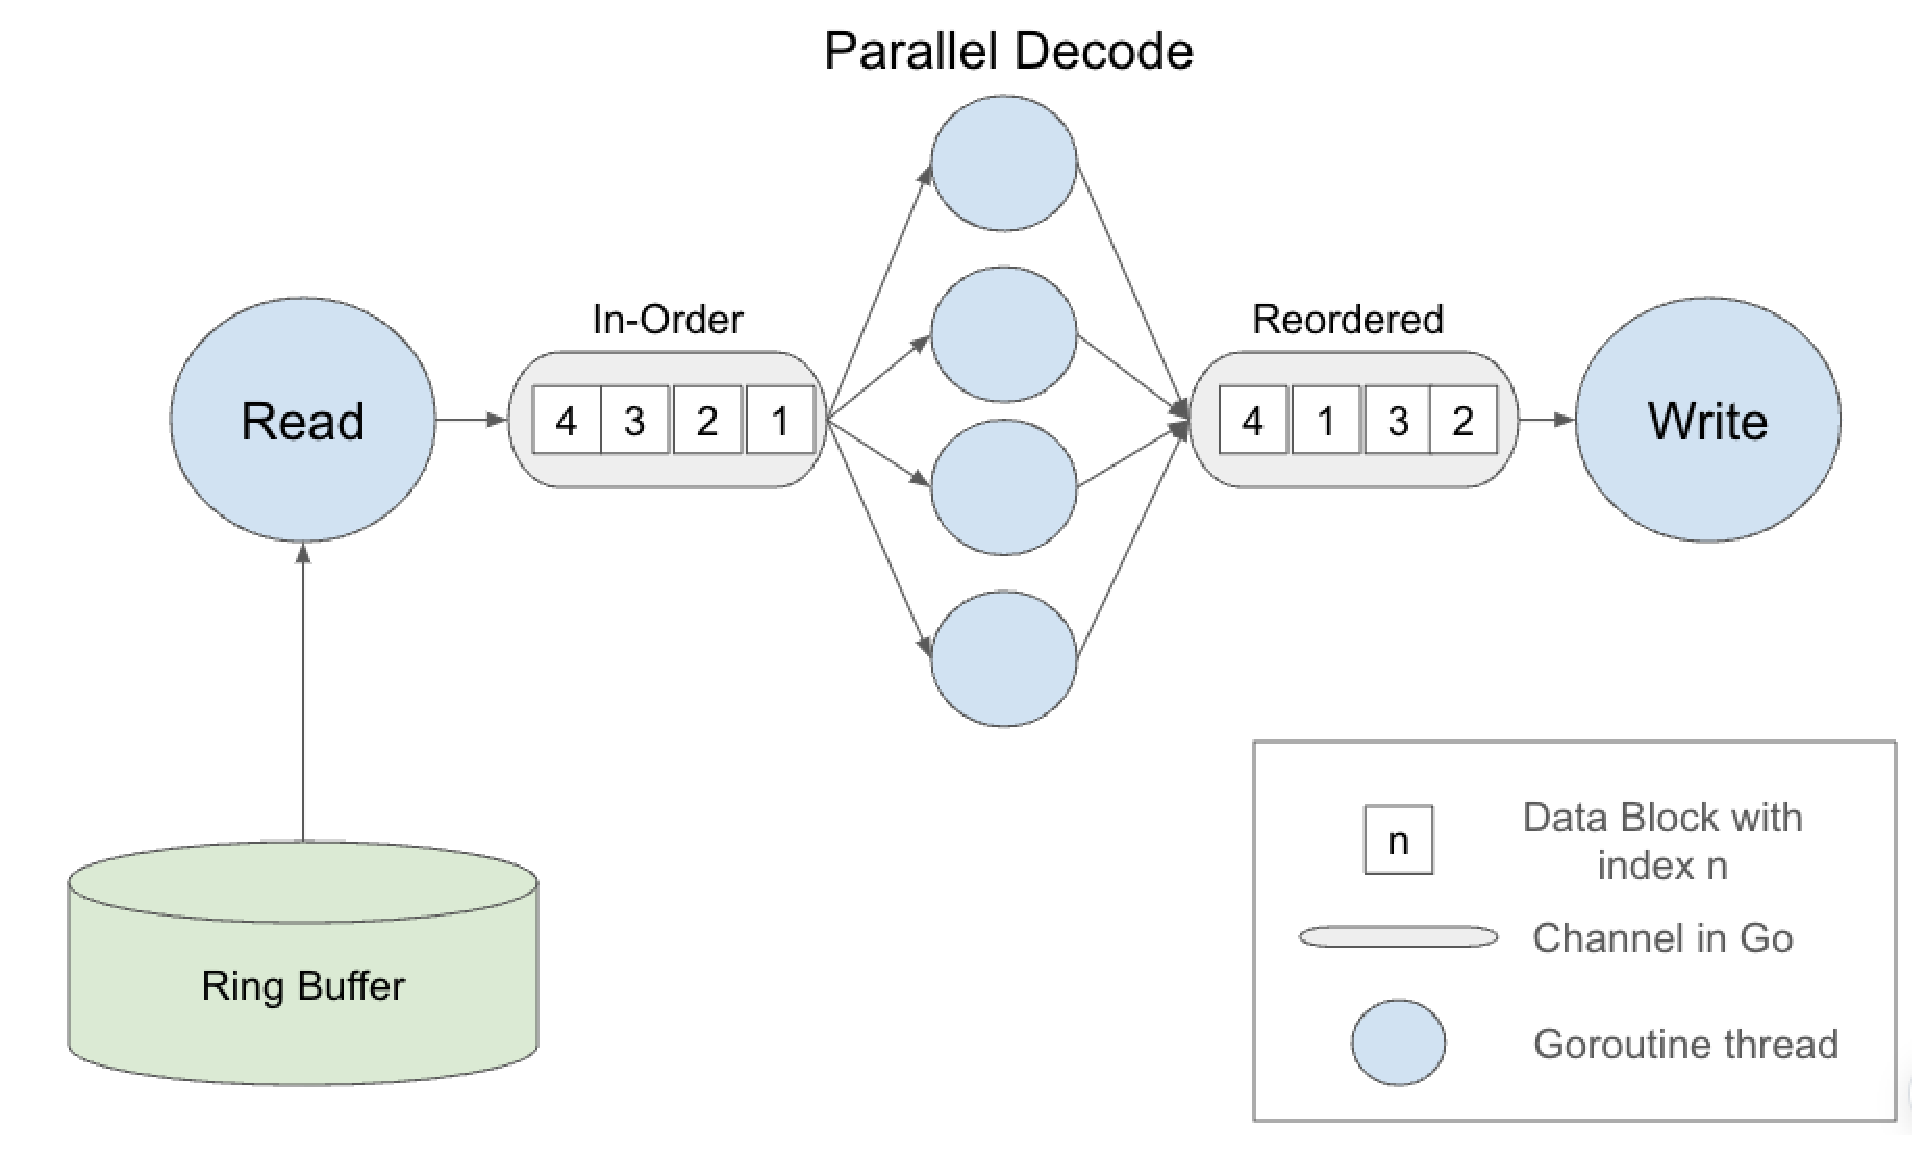
\includegraphics[width=\columnwidth]{doc/img/evac_mon_impl.eps}
  \end{center}
  \caption{foobar}
  \label{fig:evac-mon-impl}
\end{figure}



\subsection{Data Shelter}
本研究の実装では,root権限をもつユーザのみ読み書きできるディレクトリを作成し,これをData Shelterとして扱った.
ユーザ権限で実行されるランサムウェアはこのディレクトリのファイルにアクセスできないため,ランサムウェアから一定レベルの隔離が実現されている.
